\documentclass[a4paper]{article}
\usepackage{graphicx,ctable,url,amsmath}
\usepackage{subcaption}

\setlength{\parindent}{0pt}

\newcommand{\vx}{\ensuremath{\bm{\vec{x}}}}

\begin{document}

\begin{titlepage}
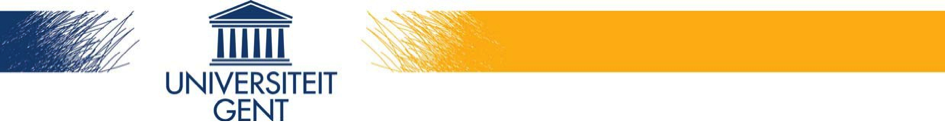
\includegraphics[width=\textwidth]{Hoofding.png}
\begin{flushleft}
UNIVERSITEIT GENT,\\
FACULTEIT INGENIEURSWETENSCHAPPEN EN ARCHITECTUUR\\
1ste master in Civil Engineering\\
Academiejaar: 2013-2014
\end{flushleft}

\begin{center}

\vspace*{\fill}

\textsc{\huge Conceptual Design}\\
[1.5cm]
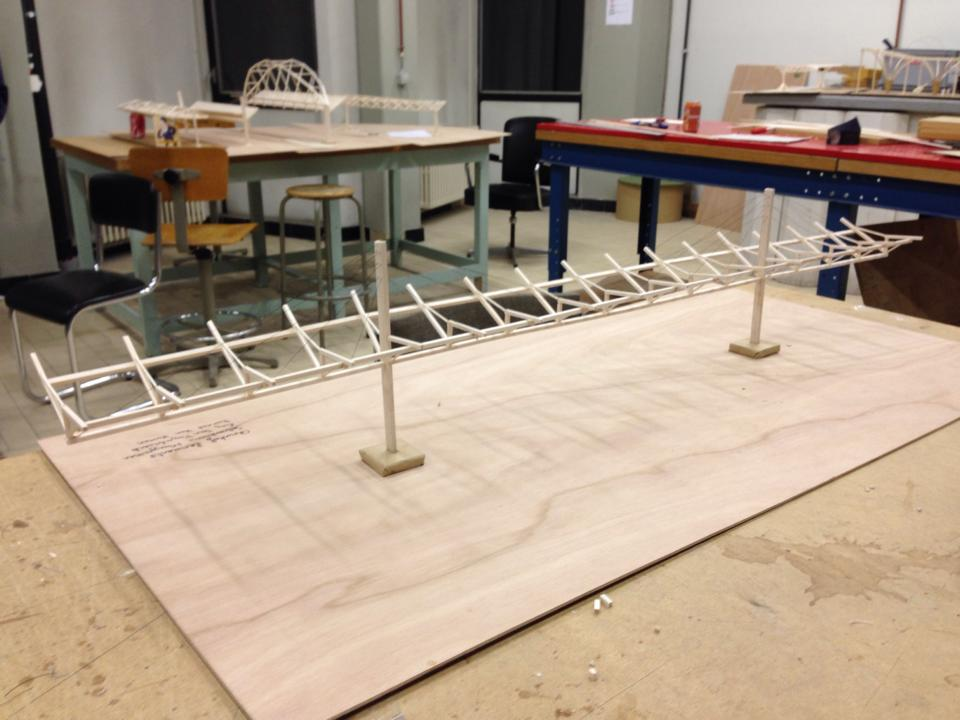
\includegraphics[width=0.7\textwidth]{ons.jpg}

\vspace{1.5cm}

\textsc{\LARGE Exercise 1: Design of a canopy structure}\\
[1cm]
Christof Lenaerts - Sebastiaan Marynissen \\
Evy Van Puymbroeck - Donaat Van Vooren - hmhm
\vspace*{\fill}

\end{center}

\begin{flushbottom}
\begin{flushleft}
Prof. ir. Bart De Pauw \\
\end{flushleft}
\end{flushbottom}

\end{titlepage}

\section{Analysis of the problem}

The goal of the first exercise is to develop a concept for a canopy structure with a larger span of $32$m, given an existing canopy structure, which was designed for a span of $8$m. This means that the functionality of the existing canopy structure should be preserved.

The existing canopy structure is depicted in figure \ref{fig:cross} and shows the dimensions, which should be more or less preserved in the extended canopy concept in order to preserve its functionality.

\begin{figure}[h]
\centering
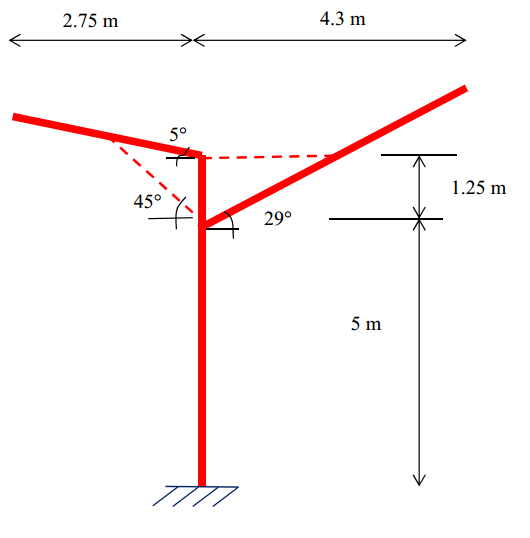
\includegraphics[width=0.4\textwidth]{crosssection.png}
\caption{Cross section of the canopy}
\label{fig:cross}
\end{figure}

The main problem when extending the canopy structure from a span of $8$m to a span of $32$m are the increased bending moments in longitudinal direction. Thus, the main concept which should be developed is a concept to counteract these bending moments. Additionally, since the increased span length also induces extra torsional moments, due to the asymmetry of the roof structure, as depicted in figure 1, and the increased leverage arm. Of course, all loads need to be transferred to the foundation through the columns, and since an increased span length results in less columns, the loads on these columns will increase as well. One understands however that this will not be a determining factor, as it can be solved easily by increasing the cross section of the columns.

\section{Development of a concept}

When dealing with increasing span lengths, one can easily get some inspiration from bridge construction. Concepts which are often used in bridge construction include external prestressing, prestressed box girder bridges, arch bridges, cable-stayed bridges, suspension bridges and so on. 

Mainly three of these concepts were taken into consideration to be translated to a canopy structure: external prestressing, an arch structure and a cable-stayed structure.

\subsection{External prestressing}

Using external prestressing, a cable would be drawn under a spatial truss which supports the roof, as depicted in figure \ref{fig:prestressing}.

\begin{figure}[h]
\centering
\begin{subfigure}[b]{0.6\textwidth}
	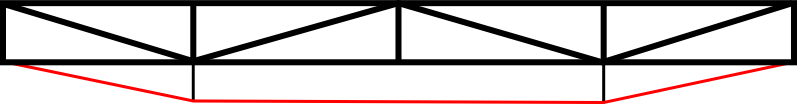
\includegraphics[width=\textwidth]{prestressing}
	\caption{Cable profile}
	\label{fig:prestressing}
\end{subfigure}
\\[1cm]
\begin{subfigure}[b]{0.6\textwidth}
	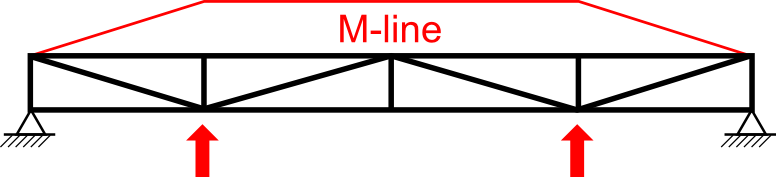
\includegraphics[width=\textwidth]{prestressing-mline}
	\caption{Bending moment line}
	\label{fig:momentline}
\end{subfigure}
\caption{Concept of external prestressing}
\end{figure}

Similar to a prestressed concrete beam this would induce upward forces in the truss, which induces a bending moment according to the relation
\[
M = \int V \mathrm{d}x
\]
as also depicted in figure \ref{fig:momentline}. Since the induced forces act upwards, this bending moment counteracts the bending moment due to the self weight and wind loads, resulting in a lower total bending moment.

This concept was rejected however, since [ja waarom eigenlijk?] Also, this concept does not include any solution to the increased torsional moments in the structure. Additionally, it was considered not aesthetically pleasing.

\subsection{Arch structure}

From an arch it is known that if its neutral line follows the profile of the bending moment line, when there was no arch, there are no bending moments in the arch. In most cases, a parabolic profile is used.

\begin{figure}[h]
\centering
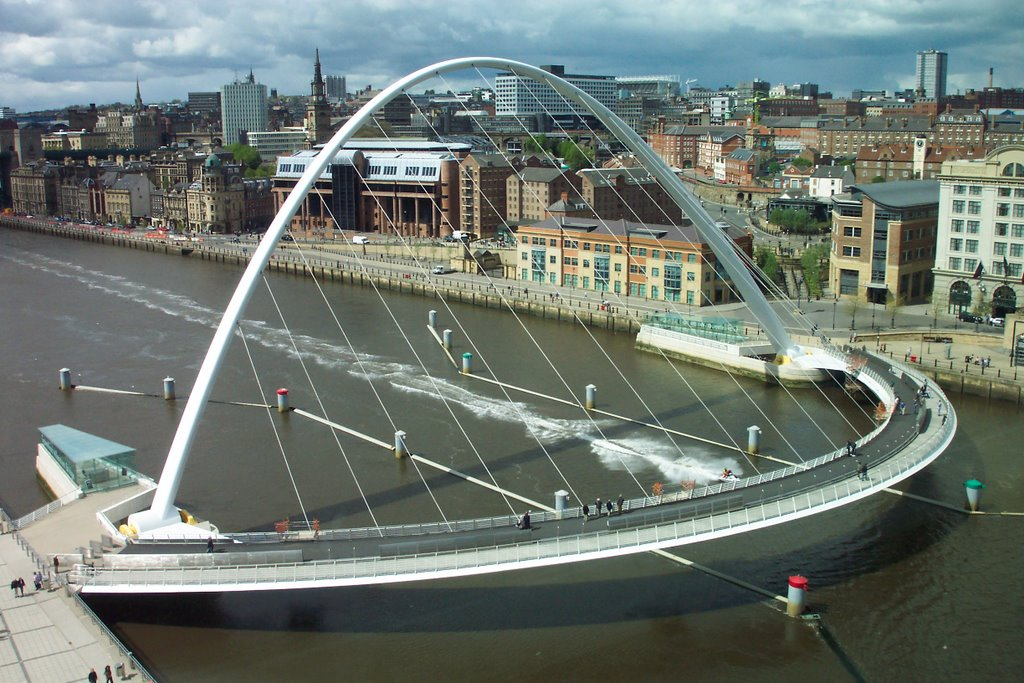
\includegraphics[width=0.7\textwidth]{gateshead.jpg}
\caption{Gateshead Millenium Bridge, Newcastle}
\label{fig:arch}
\end{figure}

The concept would be to suspend the roof with cables to the arch, similar to what was used in the Gateshead Millenium Bridge, Newcastle, depicted in figure \ref{fig:arch}. Using two rows of cables, one on each side of the arch, the concept would also be able to support the additional torsional moments.

The problem however with this concept is that arches induce horizontal thrust forces at their abutments. These additional forces should be absorbed by the columns and at the foundation as a bending moment and horizontal force. Also, an arch was considered aesthetically pleasing when there is only one arch. However, since the canopy structure exists out of multiple spans of $32$m, this would imply multiple arches next to eachother. In this light, an arch structure was rejected as suitable concept.

\subsection{Cable-stayed structure: final choice}

As a final concept, a cable-stayed concept was retained. A cable-stayed structure aims to reduce the bending moments by providing additional supports, which can be modeled as springs, as depicted in figure \ref{fig:comparison}.

\begin{figure}[h]
\begin{subfigure}[b]{\textwidth}
	\centering
	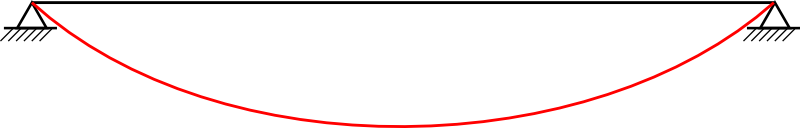
\includegraphics[width=0.6\textwidth]{simplemoment}
	\caption{Bending moments for a simply supported beam}
	\label{fig:simplemoment}
\end{subfigure}
\\[7mm]
\begin{subfigure}[b]{\textwidth}
	\centering
	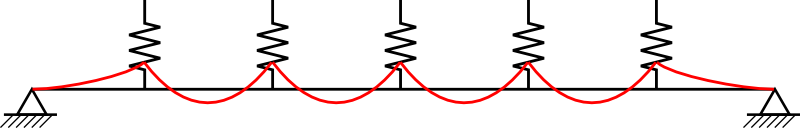
\includegraphics[width=0.6\textwidth]{cablemoment}
	\caption{Cable-stayed bending moments}
	\label{fig:simplemoment}
\end{subfigure}
\caption{Concept of cable-stayed structures}
\label{fig:comparison}
\end{figure}

Also, by using two rows of cables, the torsion due to the asymmetry of the canopy structure can be absorbed by the cables, if sufficient prestressing is added, such that the cables remain under tension at all times.

Also, to provide additional stiffness, it is chosen to weld a longitudinal beam to the columns, to provide additional stiffness in all directions. To prevent the structure to be directly supported by the columns, and for the cables to become useless, this welding should happen after the roof is fully supported by the cables.

\section{Computation in SCIA Engineer}

\section{Prediction of the deformations}

Critical note: E-modulus ratio's don't reflect real ratio's! Canopy structure only supported by the columns and not by the cables is already stable on its own!

\end{document}